\section{Computer Vision}
\subsection{Beacon Detection}
A key part of the project was the detection of the beacons to assist the dead reckoning to ensure accuracy in the localisation of the rover.
The requirements of this system are as follows:

\begin{itemize}
    \item The hardware specified on the FPGA must be able to detect each of the individual colours of the beacons (red, orange, blue)
    \item Bounding boxes must be accurately placed around each of the beacons
    \item Coordinates of corners of the boxes must be stored and passed onto the FPGA
\end{itemize}

The sample code provided for the FPGA vision system was looked at as a starting point, mainly focusing on the starter image processor implemented in Verilog (EEE\verb|_|IMGPROC.v)~\cite{ref:eebalancebug}~\cite{ref:fpga_starter}. In this Verilog module, the 24-bit "sink\verb|_|data" input from the streaming sink is broken up into separate 8-bit wires: red, green and blue. These wires are used to determine the values assigned to the 1-bit "red\verb|_|detect", "blue\verb|_|detect", "orange\verb|_|detect" and "white\verb|_|detect" wires, with the first three wires required for beacon detection and the latter wire for lane detection. These Boolean values are determined by evaluating the individual 8-bit RGB values from the video feed, for each of the beacon colours (red, orange and blue) there are a range of RGB values which are acceptable for each colour [B]. For this reason, each of the red, green and blue wires were checked against threshold values as shown below:

\begin{figure}
    \footnotesize
    \begin{minted}{systemverilog}
assign red_detect = (red[7:0] >= 8'd200) & (green[7:0] <= 8'd127) & (blue[7:0] <= 8'd127);
assign blue_detect = (red[7:0] <= 8'd127) & (green[7:0] <= 8'd127) & (blue[7:0] >= 8'd200);
assign orange_detect = (red[7:0] >= 8'd200) & (green[7:0] == 8'hff) & (blue[7:0] == 8'hff);
    \end{minted}
    \caption{Threshold values}
    \label{code:vision1}
\end{figure}

Representing threshold values in decimal was purely to make tweaking these values easier for calibration of the beacon detection.

The initial calibration without the beacons with objects of similar colours proved relatively successful in detection of colour in each respective object.

\begin{figure}
    \centering
    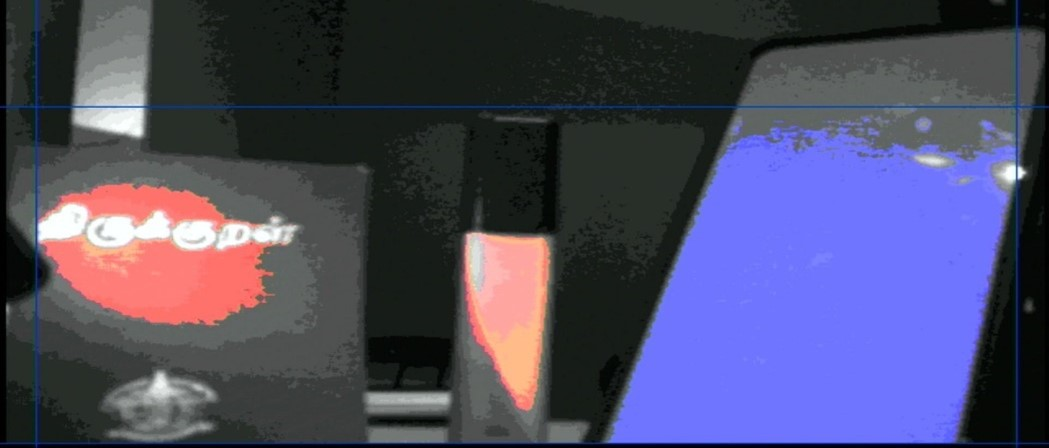
\includegraphics{images/vision-demo.jpg}
    \caption{Beacon detection}
\end{figure}

However, the image processor was unable to detect the object in its entirety due to lighting and overly strict colour detection thresholds. This was problematic as it interfered with the plan of using bounding boxes and their areas to determine the distance from the rover relative to other beacons, which cannot be done effectively if the bounding boxes do not always surround the beacon in its entirety.

In order to address this issue, the colour detection was calibrated and tested with the LED beacons, where it was learned through collaboration with the power system sub-team that the brightness of the LEDs should be limited due to bright light being detected as white light, in addition to the fact that there may be some flashing in the LEDs powered by the PV cell/ supercapacitor. Using this information, the thresholds had to be changed to allow for more robust levels of detection, which required numerous cycles of trial and error (i.e. accounting for the various shades of red, blue or orange as brightness isn’t constant throughout the beacon).

\subsection{Navigation}

The navigation system developed for the segway is a crucial part of its operation. The system has been designed to navigate autonomously through a maze environment, using a combination of Light-Dependent Resistors (LDRs), a camera, and a sophisticated wall-following algorithm. This paper will outline the techniques and technologies used in the construction of the navigation and mapping system.

The design of the segway includes the integration of LDRs on each side, which are used for wall detection. Every wall in the maze is illuminated, and the LDRs, which are sensitive to light intensity, are utilized to sense the presence of these walls. The LDRs have been carefully calibrated to a specific light intensity threshold, which is used to trigger a decision from the segway's navigation system.

\begin{figure}
    \centering
    \begin{subfigure}[b]{.45\linewidth}
        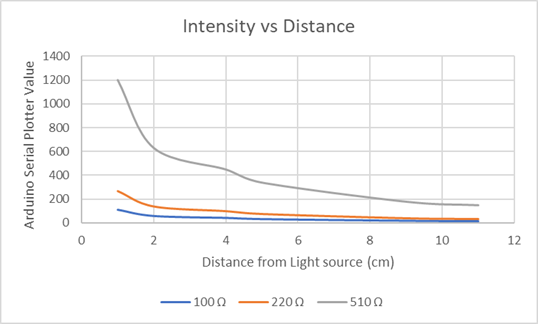
\includegraphics[width=\linewidth]{images/ldr-graph.png}
        \caption{LDR response characteristics}
    \end{subfigure}
    \begin{subfigure}[b]{0.45\linewidth}
        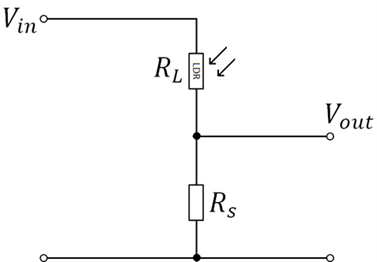
\includegraphics[width=\linewidth]{images/ldr-circuit.png}
        \caption{LDR circuit diagram}
    \end{subfigure}
    \caption{}
\end{figure}

Using a potential divider circuit, multiple resistor values were tested to measure light intensity variances as they move away from wall. A large spread of Arduinos’ measured values between varying distances from the light source (wall) was needed to set the necessary conditions for when to continue forward and when to turn, while also decreasing the margin of error.

The primary navigation algorithm employed is the right-wall following method, where the segway is programmed to follow the wall on its right side. The segway continuously checks the light intensity on its right-side LDR; if the intensity is high, implying the presence of a wall, it moves in a straight line. If the light intensity falls below the calibrated threshold, indicating the absence of a wall, it steers right until the light conditions are satisfied.

Simultaneously, the LDRs also serve a dual purpose of helping to map the maze layout. Whenever the segway encounters a junction (a point where more than two paths intersect), the LDRs detect a sudden change in light intensity by the absence of at least two walls. This is recorded as a node in the maze's graphical representation. Each node is sent to a server for processing and storage. All other pathways, representing maze corridors, are marked as weighted edges between nodes and are similarly stored on the server.

To aid the segway in maintaining accurate positioning data, coloured beacons are placed along the way. Each beacon has a pre-known location. The camera mounted on the segway recognizes these beacons and updates the segway's current location in the mapping system. This ensures a continuous update of the segway's current location in the maze, thus increasing the accuracy of the generated map.

In scenarios where the segway moves out of sight of the beacons, a technique called dead reckoning is used. Dead reckoning estimates the segway's position relative to a known starting point (the origin), based on its direction and distance travelled. This provides an additional layer of redundancy to the system, ensuring that the segway's position can be estimated even when other localization systems (like beacon recognition) are not applicable.

In conclusion, the combination of LDR sensors, a camera, and wall-following and dead-reckoning algorithms provides a comprehensive solution for the segway to navigate and map the maze. This multi-faceted approach ensures robustness, reliability, and adaptability to changing conditions within the maze, thereby enabling efficient and autonomous maze navigation and mapping.

\subsection{Dead-reckoning position estimation}

The dead-reckoning algorithm is used to estimate the segway's position relative to its starting point defined as \((0,0)\). The algorithm counts the number of steps of each motor and adjusts the estimated angle and position accordingly.

The segway turns by shutting down one motor and rotating the other, therefore the angle is estimated during a turn by using the number of steps of the outside motor as the arc of a circle.

% Diagram
\begin{figure}
    \centering
    \(\theta = \frac{360 \deg \times \text{Steps} \times \text{Distance per step} }{2 \pi \times \text{Wheelbase}}\)
    \caption{Angle estimation}
    \label{formula:angle_estimate}
\end{figure}
The position during a turn is defined by figure \ref{formula:position_estimate_turn}:

\begin{figure}
    \centering
    \(\Delta x = \frac{\text{Wheelbase}}{2} \times \sin(\theta)\)

    \(\Delta y = \frac{\text{Wheelbase}}{2} \times \cos(\theta)\)
    \caption{Position estimate during a turn}
    \label{formula:position_estimate_turn}
\end{figure}

The position during a straight line, assuming angle 0 is facing towards positive y, is defined in figure \ref{formula:position_estimate_straight}

\begin{figure}
    \centering
    \(\Delta x = \text{Steps} \times \text{Distance per step} \times \sin(\theta)\)

    \(\Delta y = \text{Steps} \times \text{Distance per step} \times \cos(\theta)\)
    \caption{Position estimate in a straight line}
    \label{formula:position_estimate_straight}
\end{figure}


\subsection{Testing}

Three different types of light sensors are tested to see which was most suited for the task of navigating. A high sensitivity to light and a steady variance in light detected depending on distance from light source are needed in the design. A GL5528 photoresistor was tested first:

%Photoresistor figure

\begin{figure}
    \centering
    \begin{subfigure}[b]{.2\linewidth}
        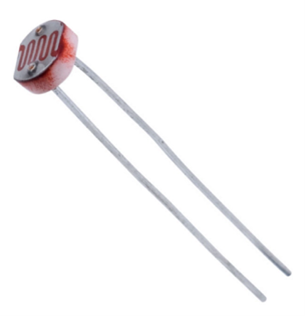
\includegraphics[width=\linewidth]{images/photoresistor.png}
        \caption{Photoresistor}
    \end{subfigure}
    \hspace{2cm}
    \begin{subfigure}[b]{.4\linewidth}
        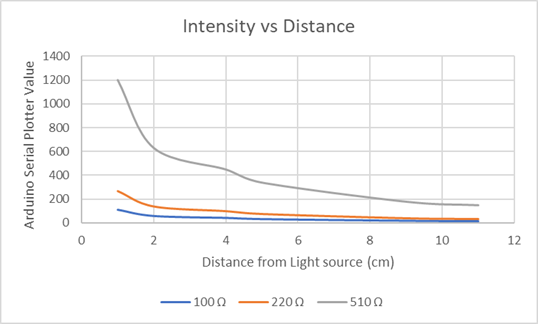
\includegraphics[width=\linewidth]{images/ldr-graph.png}
        \caption{Phototransistor response characteristics}
    \end{subfigure}
    \caption{}
\end{figure}


The GL5528 photoresistor proved to have great results when it is paired up with a 510\(\Omega\) resistor in a potential divider circuit.

An SFH 300 phototransistor was tested next, the idea behind choosing this one was that it would be able to detect light from more directions due to its design:

%Phototransistor figure 
\begin{figure}
    \centering
    \begin{subfigure}[b]{0.2\linewidth}
        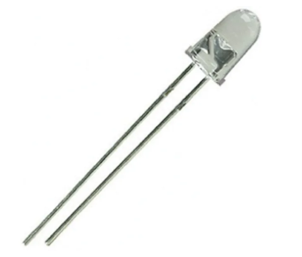
\includegraphics[width=\linewidth]{images/phototransistor.png}
        \caption{Phototransistor}
    \end{subfigure}
    \hspace{2cm}
    \begin{subfigure}[b]{0.4\linewidth}
        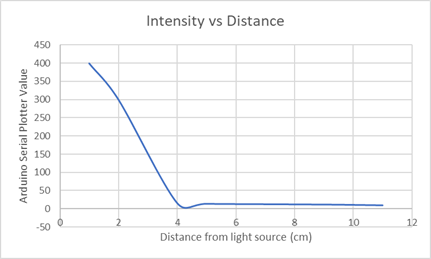
\includegraphics[width=\linewidth]{images/phototransistor-graph.png}
        \caption{Phototransistor response characteristics}
    \end{subfigure}
    \caption{}
\end{figure}

The issue with the phototransistor was that the variance was not steady and it would barely detect anything if it was not immediately next to the light source.

Finally, the last component that was tested was a photoresistor sensor module. The idea behind trying this was to save space on the breadboard as it did not require the use of a potential divider circuit:

%Module figure
\begin{figure}
    \centering
    \begin{subfigure}[b]{0.2\linewidth}
        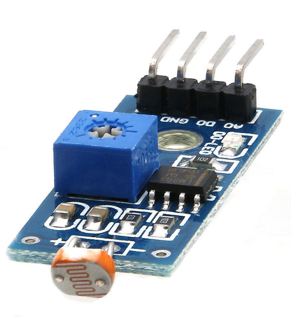
\includegraphics[width=\linewidth]{images/photomodule.png}
        \caption{Photoresistor module}
    \end{subfigure}
    \hspace{2cm}
    \begin{subfigure}[b]{0.4\linewidth}
        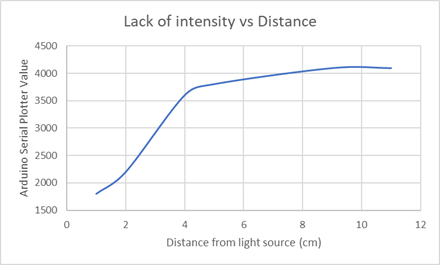
\includegraphics[width=\linewidth]{images/photomodule-graph.png}
        \caption{Photoresistor module response characteristics}
    \end{subfigure}
    \caption{}
\end{figure}

Again, the issue with this was that it barely detected changes in conditions until the light source was very close. This performed better than the SFH 300 but worse than the GL5528. In the end, the GL5528 was chosen as it was the best suited for gauging its distance to the light source. This property would be heavily relied on in the navigation.

\subsection{Algorithm}

When searching for an algorithm that computes the shortest path in a graph,  there were a breadth of choices. These include Dijkstra's algorithm, Bellman–Ford algorithm, A* search algorithm, Floyd–Warshall algorithm, Johnson's algorithm. Now these algorithms needed to be assessed with respect to their time-complexities.
\begin{figure}
    \centering
    \begin{tabular}{ | p{2cm} | p{2cm} | p{2cm} | p{2cm} | p{2cm} | p{2cm} |}

        \hline
        Algorithm           & Dijkstra     & Bellman-Ford & A* search          & Floyd-Warshall & Johnson's           \\
        \hline
        Space complexity    & \(O(E)\)       & \(O(E)\)       & Heuristic Function & \(O(V^2)\)       & Heuristic Function  \\
        \hline
        Time complexity     & \(O(V^2)\)     & \(O(VE)\)      & Heuristic Function & \(O(V^3)\)       & \(O(V^2 \log V + VE)\) \\
        \hline
        \multicolumn{3}{|c|}{V = Vertices} & \multicolumn{3}{c|}{E = Edges} \\
        \hline
    \end{tabular}
    \caption{Time and space complexities of various algorithms}
    \label{tbl:algorithm-complexities}
\end{figure}

The use of Dijkstra's algorithm was proposed for a non-orthogonal maze traversal problem, where the start and end points are diagonally opposite. The reason is as follows:

Dijkstra's algorithm was a formidable option for our problem set, particularly when the uniform cost and non-negativity are considered of our edge weights. While the A* algorithm's uses of a heuristic function may seem appealing at first glance, it’s worth considering that Dijkstra’s has an inherent advantage in dealing with graphs that don't provide additional heuristic information. Dijkstra's algorithm operates by treating every direction as equally potential, thus exploring the entire graph uniformly.

Contrary to the A* search algorithm, which heavily relies on a heuristic function, Dijkstra's algorithm does not need any heuristic information to guide the search, and this has the benefit of a more thorough exploration of the graph which is advantageous in situations where the heuristics may not provide an optimal solution.

As for the Bellman-Ford algorithm, it is less efficient than Dijkstra's algorithm when considering time complexities, as there will be less vertices than edges, making this a less practical choice for our situation. It is also usually reserved for scenarios where edge weights can be negative, which is not the case for our maze.

Floyd-Warshall and Johnson's algorithms, meanwhile, are designed to compute the shortest paths between all pairs of nodes. In our specific problem where the only need is to determine the shortest path from a single source to a single target, these algorithms seem to be an overuse of resources.

Dijkstra's algorithm, in its simplicity and uniformity, shines in this particular scenario where there is only a single source and a single target. It's an efficient algorithm, both in terms of time and space complexities, and offers a reliable method of finding the shortest path in a graph. Thus, the use of Dijkstra's algorithm is chosen in our maze traversal.